\chapter{Chapter title}
\label{sec:firstchap}
\thispagestyle{myheadings}

%This command will reset all acronyms, so that when you call an acronym for the first time, it will display the long form followed by the short form in parenthesis.  If you call this at the beginning of every chapter, it will display the long-form acronym again the first time you use that acronym within the chapter.  Personally, I think this is a very good idea, especially if you define an acronym in chapter 1 and then don't discuss it again until chapter 4, it makes sense to spell it out again.
\glsresetall

Example reference to Section \ref{sec:fakesection}.  Example reference to Figure \ref{fig:fakefigure}.  Example reference to Equation~\ref{eqn:fakeequation}.  Example reference to better Equation~\ref{eqn:velocity_dispersion}.  Example reference to Table~\ref{table:deluxetableexample}.  Example reference to Table~\ref{table:longtableexample}.  Example parenthetical citation: \citep[e.g][for example]{gosling_1993}.   Example textual citation to \citet[][]{gosling_1993}.  Example call of a \gls{tla}.  Additionally, \gls{oah}.  If you are referring to plural \glspl{tla}, it can also be done, and the glossary package will simply add an 's' to the end of the acronym.  If you have something trickier, that can also be done.  For example, if you have two \glspl{sn}, as long as you define it in the main thesis.tex file, it comes out with the correct first usage plural.  And if we want to refer to it again, we can (like here:  \glspl{sn}) and it will be plural (or it can be singular as well:  \gls{sn}).  Here is an example of using a \gls{twaa}.  Further uses look like \gls{twaa}.  And using a symbol as an acronym can also be done, for example \gls{sdss}.  I want \gls{sdss} to be italicized and I always forget, so I made it a command.  Further information about the Glossaries package can be found at \url{http://www.math.washington.edu/tex-archive/macros/latex/contrib/glossaries/glossaries-user.pdf} or at the CTAN site: \url{http://ctan.org/tex-archive/macros/latex/contrib/glossaries} where you can download and install the package.  Also, that was an example of using the hyperref package and the url tag.  As we can see, the hyperref package doesn't always play nice with the margins of the document.  I highly recommend checking every hyperref call you make at some point.  When you print, the boxes don't show up, but it won't help with the page format.  Setting breaklinks=True doesn't seem to help.  So if you have this issue in your dissertation, I would recommend turning off the hyperref package.  Hopefully that will help.  Otherwise, take a look at the hyperref documentation.

Lorem ipsum dolor sit amet, consectetur adipiscing elit. Praesent nec velit magna. In vehicula accumsan blandit. Duis vestibulum eros et ante posuere et pharetra nibh dapibus. Pellentesque quis nibh vestibulum urna fermentum convallis. Duis ultricies felis eget orci sodales sed varius ante facilisis. Vivamus nec lorem nulla. Donec id quam id arcu fringilla euismod. Etiam ullamcorper posuere ipsum, vel egestas ipsum bibendum faucibus. Proin volutpat dolor vel nulla egestas in ultricies mi pellentesque. Vivamus ut nulla ligula.

Vestibulum sed ante leo, et malesuada massa. Aenean vulputate dictum auctor. Nunc dignissim nibh ut lorem placerat eu convallis magna fermentum. Nullam ut magna in libero pharetra semper. Phasellus et odio sit amet eros facilisis dignissim. Curabitur tempor aliquet purus, ac blandit sem viverra ac. Vivamus non leo augue, ac semper orci. Integer non felis et arcu commodo tristique. Donec est justo, vehicula in dapibus quis, molestie nec elit. Mauris non congue neque. Duis id justo id lorem porta lobortis. Proin dapibus commodo interdum. Sed tincidunt lobortis nisl eu mollis.

%#################################################################################################
%#################################################################################################
%Section
%#################################################################################################
%#################################################################################################

\section{Second Section}
\label{sec:fakesection}
Lorem ipsum dolor sit amet, consectetur adipiscing elit. Praesent nec velit magna. In vehicula accumsan blandit. Duis vestibulum eros et ante posuere et pharetra nibh dapibus. Pellentesque quis nibh vestibulum urna fermentum convallis. Duis ultricies felis eget orci sodales sed varius ante facilisis. Vivamus nec lorem nulla. Donec id quam id arcu fringilla euismod. Etiam ullamcorper posuere ipsum, vel egestas ipsum bibendum faucibus. Proin volutpat dolor vel nulla egestas in ultricies mi pellentesque. Vivamus ut nulla ligula.

%#################################################################################################
%#################################################################################################

\subsection{Subsection}
\label{sec:fakesubsec}

\subsubsection*{Subsubsection}
Lorem ipsum dolor sit amet, consectetur adipiscing elit. Praesent nec velit magna. In vehicula accumsan blandit. Duis vestibulum eros et ante posuere et pharetra nibh dapibus. Pellentesque quis nibh vestibulum urna fermentum convallis. Duis ultricies felis eget orci sodales sed varius ante facilisis. Vivamus nec lorem nulla. Donec id quam id arcu fringilla euismod. Etiam ullamcorper posuere ipsum, vel egestas ipsum bibendum faucibus. Proin volutpat dolor vel nulla egestas in ultricies mi pellentesque. Vivamus ut nulla ligula.

\begin{figure}[!hbtp]
\begin{center}
\capstart  %When you click on the hyperlink, it will bring you to the top of the figure instead of the top of the caption.  Personal preference, but I much prefer it this way...
\includegraphics[height=\linewidth, angle=0]{chapter1/figures/bunny.ps}
\caption[Caption for `list of figures' page here]{Caption to be shown under the figure here}
\label{fig:fakefigure}
\end{center}
\end{figure}

\begin{equation}
\label{eqn:fakeequation}
R_{L} = \frac{mv_{\perp}}{qB}
\end{equation}

Of course, I have to add my own equation, because the above equation doesn't pertain to me.  The velocity dispersion of a galaxy cluster is defined as:
\begin{equation}
\label{eqn:velocity_dispersion}
\sigma_r = \langle \left(v_r - \langle v_r\rangle \right)^2 \rangle^{1/2}
\end{equation}
which only holds as long as the distribution is Gaussian, i.e.:
\begin{equation}
\label{eqn:gauss}
p\left(v_r\right)dv_r = \frac{1}{\sigma_r \sqrt[2]{2 \pi}} e^{\frac{-\left(v_r - \langle v_r \rangle \right)^2}{2 \sigma_r^2}}d v_r
\end{equation}
where $p\left(v_r \right) d v_r$ is the probability that the velocity falls between $v_r$ and $v_r + dv_r$.


{\noindent}Lorem ipsum dolor sit amet, consectetur adipiscing elit. Praesent nec velit magna. In vehicula accumsan blandit. Duis vestibulum eros et ante posuere et pharetra nibh dapibus. Pellentesque quis nibh vestibulum urna fermentum convallis. Duis ultricies felis eget orci sodales sed varius ante facilisis. Vivamus nec lorem nulla. Donec id quam id arcu fringilla euismod. Etiam ullamcorper posuere ipsum, vel egestas ipsum bibendum faucibus. Proin volutpat dolor vel nulla egestas in ultricies mi pellentesque. Vivamus ut nulla ligula.  

Here is an example of a deluxetable (Table~\ref{table:deluxetableexample}).  You can use deluxetable as long as you don't use the array package in the main thesis.tex file.  The choice is yours.  This is a very intricate deluxetable, with both numerical and alphabetical references.  There are also tablecomments in addition to the table caption.  The only issue with deluxetable is that if the table spans multiple pages, each page of the table gets added to the list of tables as a separate entry with the same name.  This doesn't particularly bother me, but if it bothers you, the other option is to use longtable.  An example longtable (provided by Susanna Finn) is shown below.
\begin{deluxetable}{lcccccrrccccrcc}
\tabletypesize{\tiny}
\tablewidth{0pt}
\tablecolumns{15}
\tablecaption{Sources located in rich cluster environments} %As far as I can tell, you can't define separate captions for the list of tables and what is actually shown above the table, at least not within the 
\tablehead{\colhead{Source Name}&
		  \colhead{Smpl\tablenotemark{1}}&
		  \colhead{$\alpha$}&
		  \colhead{$\delta$}&
		  \colhead{$m_r$}&
		  \colhead{$M_r$}&
		  \colhead{S}&
		  \colhead{Angle}&
		  \colhead{$P_{1440\: \rm MHz}$}&
		  \colhead{FR\tablenotemark{2}}&
		  \colhead{FR\tablenotemark{3}}&
		  \colhead{$z$}&
		  \colhead{N$^{-19}_{1.0}$}&
		  \colhead{$f_c$}&
		  \colhead{Abell}
		  \cr
		   & & & &
		  \colhead{(mag)}&
		  \colhead{(mag)}& 
		  \colhead{(mJy)}&
		  \colhead{(deg)}&
		  \colhead{(W Hz$^{-1}$)}&
		   & & & & &
		  \cr
		  \colhead{(1)}&
		  \colhead{(2)}&
		  \colhead{(3)}&
		  \colhead{(4)}&
		  \colhead{(5)}&
		  \colhead{(6)}&
		  \colhead{(7)}&
		  \colhead{(8)}&
		  \colhead{(9)}&
		  \colhead{(10)}&
		  \colhead{(11)}&
		  \colhead{(12)}&
		  \colhead{(13)}&
		  \colhead{(14)}&
		  \colhead{(15)}}
%The table can be rotated into landscape using the rotate command below.
%\rotate
\startdata
J002859.3$+$002000 & S & 00:28:59.38 & $+00$:20:00.6 & 17.12 & $-23.40$ & 19.8 & 169.5 & 2.77e+24 & I & I & 0.222\tablenotemark{a} & 61 & 1.00 & \nodata\\
J005625.7$-$011543 & V & 00:56:25.70 & $-01$:15:43.0 & 13.36 & $-24.48$ & 515.3 & 85.0 & 7.60e+24 & I & I & 0.078\tablenotemark{b} & 52 & 1.00 & A0119\\
J005702.0$-$005230 & A & 00:57:02.07 & $-00$:52:30.7 & 13.41 & $-23.11$ & 72.5 & 147.2 & 3.29e+23 & I & I & 0.044\tablenotemark{a} & 53 & 1.00 & A0119\\
J005702.1$-$005231 & V & 00:57:02.10 & $-00$:52:31.0 & 13.41 & $-23.11$ & 72.5 & 147.0 & 3.29e+23 & I & I & 0.044\tablenotemark{a} & 53 & 1.00 & A0119\\
J010242.5$-$005032 & V & 01:02:42.50 & $-00$:50:32.0 & 17.46 & $-23.54$ & 66.5 & 87.0 & 1.33e+25 & I & I & 0.261\tablenotemark{b} & 64 & 1.00 & \nodata\\
J010456.5$+$000423 & V & 01:04:56.50 & $+00$:04:23.0 & 18.26 & $-23.26$ & 83.4 & 8.0 & 2.50e+25 & I & I & 0.312\tablenotemark{b} & 206 & 1.37 & \nodata\\
J011403.1$-$011058 & V & 01:14:03.10 & $-01$:10:58.0 & 16.90 & $-23.15$ & 16.5 & 139.0 & 1.59e+24 & I & I & 0.187\tablenotemark{a} & 55 & 1.00 & \nodata\\
J011403.1$-$011057 & A & 01:14:03.15 & $-01$:10:58.0 & 16.90 & $-23.15$ & 16.5 & 138.9 & 1.59e+24 & I & I & 0.187\tablenotemark{a} & 55 & 1.00 & \nodata\\
J011633.3$-$092753 & S & 01:16:33.38 & $-09$:27:53.3 & 18.17 & $-22.74$ & 22.1 & 179.2 & 4.13e+24 & I & I & 0.253\tablenotemark{b} & 47 & 1.00 & \nodata\\
J013503.8$+$011325 & S & 01:35:03.81 & $+01$:13:25.3 & 18.90 & $-23.08$ & 20.7 & 175.9 & 8.56e+24 & I & I & 0.359\tablenotemark{b} & 122 & 1.91 & \nodata\\
J022736.7$-$005253 & V & 02:27:36.70 & $-00$:52:53.0 & 20.26 & $-19.24$ & 69.7 & 85.0 & 4.84e+24 & II & II? & 0.161\tablenotemark{b} & 49 & 1.00 & \nodata\\
J023027.9$+$010847 & A & 02:30:27.96 & $+01$:08:47.2 & 17.45 & $-23.65$ & 130.9 & 87.8 & 2.77e+25 & I & I & 0.267\tablenotemark{a} & 103 & 1.05 & \nodata\\
J023028.1$+$010850 & V & 02:30:28.10 & $+01$:08:50.0 & 17.45 & $-23.65$ & 130.9 & 88.0 & 2.77e+25 & I & I & 0.267\tablenotemark{a} & 108 & 1.05 & \nodata\\
J030259.5$-$001136 & V & 03:02:59.50 & $-00$:11:36.0 & 17.29 & $-22.38$ & 63.8 & 97.0 & 4.23e+24 & I & I & 0.158\tablenotemark{a} & 49 & 1.00 & \nodata\\
J072244.7$+$302842 & S & 07:22:44.71 & $+30$:28:42.4 & 19.38 & $-22.90$ & 15.8 & 176.5 & 7.44e+24 & I & I & 0.380\tablenotemark{b} & 106 & 2.47 & \nodata\\
J072248.4$+$412921 & A & 07:22:48.43 & $+41$:29:21.2 & 15.60 & $-22.78$ & 31.7 & 146.2 & 7.37e+23 & I & I & 0.097\tablenotemark{b} & 42 & 1.00 & \nodata
\enddata
\tablecomments{A question mark in Col. 11 represents a dubious visual FR I/II classification.  Three successive question marks represent an inability to visually classify the radio source as either FR I or II.}
\tablenotetext{1}{The sample each source belongs to:  V = visual bent sample, A = auto bent sample, and S = straight sample.}
\tablenotetext{2}{FR type determined following Ledlow \& Owen (1996).}
\tablenotetext{3}{FR type determined visually.}
\tablenotetext{a}{The redshift comes from a spectroscopic measurement.}
\tablenotetext{b}{The redshift comes from a photometric measurement.}
\tablenotetext{c}{The difference in redshift between the identified Abell cluster (from NED) and the radio cluster is greater than $1500$ km s$^{-1}$.}
\tablenotetext{d}{The Abell cluster does not have a confirmed redshift in NED.}
\label{table:deluxetableexample}
\end{deluxetable}

This is an example of the longtable table format in action (Table~\ref{table:longtableexample}).  There are lots of cool things it can do (except for mix alphabetical and numerical footnotes or do tablecomments), and I highly suggest reading up on it if you have further questions.  Some relevant information is found at:  \url{http://www2.astro.psu.edu/gradinfo/psuthesis/longtable.html} and at:  \url{http://texblog.org/2011/05/15/multi-page-tables-using-longtable/}.
		\begin{landscape}%[!htp]
		\begin{center}
		\begin{longtable}{lccccrcccc}%[!htp]
	\caption[Fourth Quadrant IRDC Candidates Detected in CS]{Fourth Quadrant IRDC Candidates Detected in CS}\label{table:longtableexample}\\
\hline \hline \\[-2ex]
	\multicolumn{1}{c}{IRDC Candidate$^{a}$} &%\dagger}$} &%$^{\dagger}$} & 
%	\multicolumn{1}{c}{Core} &
	\multicolumn{2}{c}{Coordinates} &
	\multicolumn{1}{c}{Peak} &
	\multicolumn{1}{c}{Peak T$_A^*$} &
	\multicolumn{1}{c}{Velocity} &
	\multicolumn{1}{c}{FWHM} &
	\multicolumn{1}{c}{Int. Int.$^{b}$} &%\dagger\dagger}$} &
	\multicolumn{1}{c}{R$_{Gal}\,^{c}$} &%\ddag}$} &
	\multicolumn{1}{c}{D$_{near}\,^{c}$} \\%\ddag}$} \\%&
%	\multicolumn{1}{c}{Two Velocity} \\%&
	\multicolumn{1}{c}{{\scriptsize \it MSXDC}} &
%	\multicolumn{1}{c}{} & %Min\tablenotemark{d}} &
	\multicolumn{1}{c}{{\scriptsize \it $\ell$\degr}} & %\scriptsize{\it{l}\degr}} & %Max\tablenotemark{d}} &
	\multicolumn{1}{c}{\scriptsize {\it{b}\degr}} &
	\multicolumn{1}{c}{Contrast} &
	\multicolumn{1}{c}{{\scriptsize \it K}} &
	\multicolumn{1}{c}{{\scriptsize \it km s$^{-1}$}} &
	\multicolumn{1}{c}{{\scriptsize \it km s$^{-1}$}} &
	\multicolumn{1}{c}{{\scriptsize \it K\kms}} &
	\multicolumn{1}{c}{{\scriptsize \it kpc}} &
	\multicolumn{1}{c}{{\scriptsize \it kpc}} \\
	\multicolumn{1}{c}{(1)} &
	\multicolumn{1}{c}{(2)} & %\scriptsize{\it{l}\degr}} & %Max\tablenotemark{d}} &
	\multicolumn{1}{c}{(3)} &
	\multicolumn{1}{c}{(4)} &
	\multicolumn{1}{c}{(5)} &
	\multicolumn{1}{c}{(6)} &
	\multicolumn{1}{c}{(7)} &
	\multicolumn{1}{c}{(8)} &
	\multicolumn{1}{c}{(9)} &
	\multicolumn{1}{c}{(10)}\\[0.5ex] \hline \\[-1.8ex]
	\endfirsthead
	\multicolumn{10}{c}{{\tablename} \thetable{} -- Continued} \\[0.5ex]
	\hline \hline \\[-2ex]
	\multicolumn{1}{c}{IRDC Candidate$^{a}$} & %\dagger}$} & 
%	\multicolumn{1}{c}{Core} &
	\multicolumn{2}{c}{Coordinates} &
	\multicolumn{1}{c}{Peak} &
	\multicolumn{1}{c}{Peak T$_A^*$} &
	\multicolumn{1}{c}{Velocity} &
	\multicolumn{1}{c}{FWHM} &
	\multicolumn{1}{c}{Int. Int.$^{b}$} &%\dagger\dagger}$} &
	\multicolumn{1}{c}{R$_{Gal}\,^{c}$} &%\ddag}$} &
	\multicolumn{1}{c}{D$_{near}\,^{c}$}\\%\ddag}$} \\%&
%	\multicolumn{1}{c}{Two Velocity} \\%&
	\multicolumn{1}{c}{{\scriptsize \it MSXDC}} &
%	\multicolumn{1}{c}{} & %Min\tablenotemark{d}} &
	\multicolumn{1}{c}{{\scriptsize \it $\ell$\degr}} & %\scriptsize{\it{l}\degr}} & %Max\tablenotemark{d}} &
	\multicolumn{1}{c}{{\scriptsize \it{b}\degr}} &
	\multicolumn{1}{c}{Contrast} &
	\multicolumn{1}{c}{{\scriptsize \it K}} &
	\multicolumn{1}{c}{{\scriptsize \it km s$^{-1}$}} &
	\multicolumn{1}{c}{{\scriptsize \it km s$^{-1}$}} &
	\multicolumn{1}{c}{{\scriptsize \it K\kms}} &
	\multicolumn{1}{c}{{\scriptsize \it kpc}} &
	\multicolumn{1}{c}{{\scriptsize \it kpc}}\\
	\multicolumn{1}{c}{(1)} &
%	\multicolumn{1}{c}{} & %Min\tablenotemark{d}} &
	\multicolumn{1}{c}{(2)} & %\scriptsize{\it{l}\degr}} & %Max\tablenotemark{d}} &
	\multicolumn{1}{c}{(3)} &
	\multicolumn{1}{c}{(4)} &
	\multicolumn{1}{c}{(5)} &
	\multicolumn{1}{c}{(6)} &
	\multicolumn{1}{c}{(7)} &
	\multicolumn{1}{c}{(8)} &
	\multicolumn{1}{c}{(9)} &
	\multicolumn{1}{c}{(10)}  \\[0.5ex] \hline \\[-1.8ex]%\multicolumn{1}{c}{Components?}
\endhead
G282.28$-$00.73	(a)		&	282.29	&	$-$0.74	&	0.39	&	0.43	&	\phn\phn\phn5.9	\phn	&	\phn1.7	&	\phn0.79	&	\phn8.44	&	\phn0.29	\\
																						
G287.17$-$00.38	(a)		&	287.18	&	$-$0.38	&	0.40	&	0.22	&	\phn$-$21.3	\phn	&	\phn1.2	&	\phn0.28	&	\phn8.12	&	\phn2.51	\\
																						
G291.40$-$00.19	(a)		&	291.40	&	$-$0.19	&	0.76	&	0.57	&	\phn\phn$-$6.1	\phn	&	\phn1.6	&	\phn0.97	&	\phn8.10	&	\phn1.37	\\
G293.34$-$00.85	(a)	*	&	293.35	&	$-$0.86	&	0.42	&	0.68	&	\phn$-$27.6	\phn	&	\phn1.4	&	\phn1.02	&	\phn7.80	&	\phn3.37	\\
G293.34$-$00.85	(a)	*	&	293.35	&	$-$0.86	&	0.42	&	0.30	&	\phn$-$23.1	\phn	&	\phn0.9	&	\phn0.30	&	\phn7.80	&	\phn3.37	\\
																						
																						
G305.51+00.76	(a)		&	305.52	&	\phn0.77	&	0.36	&	0.70	&	\phn$-$28.1	\phn	&	\phn3.2	&	\phn2.35	&	\phn7.38	&	\phn2.36	\\
G306.57+00.34	(a)		&	306.58	&	\phn0.34	&	0.39	&	0.13	&	\phn$-$45.2	\phn	&	\phn7.3	&	\phn1.02	&	\phn6.84	&	\phn4.57	\\
G306.65$-$00.21	(a)		&	306.67	&	$-$0.21	&	0.38	&	2.01	&	\phn$-$27.4	\phn	&	\phn1.0	&	\phn2.04	&	\phn7.39	&	\phn2.22	\\
G306.92$-$00.05	(a)		&	306.92	&	$-$0.06	&	0.45	&	1.05	&	\phn$-$28.4	\phn	&	\phn1.4	&	\phn1.51	&	\phn7.36	&	\phn2.30	\\
																						
G308.39$-$00.18	(a)		&	308.40	&	$-$0.18	&	0.43	&	0.32	&	\phn$-$25.0	\phn	&	\phn2.0	&	\phn0.69	&	\phn7.45	&	\phn1.94	\\
G309.14$-$00.16	(a)		&	309.14	&	$-$0.15	&	0.52	&	0.46	&	\phn$-$45.0	\phn	&	\phn3.8	&	\phn1.85	&	\phn6.80	&	\phn3.70	\\
G309.34$-$00.69	(a)		&	309.35	&	$-$0.71	&	0.36	&	0.35	&	\phn$-$49.7	\phn	&	\phn4.6	&	\phn1.71	&	\phn6.65	&	\phn4.39	\\
G309.42$-$00.64	(a)		&	309.42	&	$-$0.64	&	0.46	&	0.40	&	\phn$-$42.2	\phn	&	\phn3.1	&	\phn1.32	&	\phn6.88	&	\phn3.33	\\
																						
G312.87$-$00.66	(a)		&	312.88	&	$-$0.66	&	0.35	&	0.27	&	\phn$-$51.0	\phn	&	\phn2.6	&	\phn0.74	&	\phn6.52	&	\phn3.85	\\
G313.70$-$00.31	(a)	*	&	313.68	&	$-$0.31	&	0.54	&	0.22	&	\phn$-$39.4	\phn	&	\phn2.3	&	\phn0.51	&	\phn6.89	&	\phn2.76	\\
G313.70$-$00.31	(a)	*	&	313.68	&	$-$0.31	&	0.54	&	0.30	&	\phn$-$44.1	\phn	&	\phn2.3	&	\phn0.69	&	\phn6.73	&	\phn3.13	\\
G313.70$-$00.31	(b)		&	313.70	&	$-$0.30	&	0.53	&	0.46	&	\phn$-$44.2	\phn	&	\phn4.2	&	\phn2.05	&	\phn6.73	&	\phn3.14	\\
G313.70$-$00.31	(c)		&	313.74	&	$-$0.30	&	0.44	&	0.80	&	\phn$-$44.3	\phn	&	\phn3.5	&	\phn2.98	&	\phn6.72	&	\phn3.15	\\
G313.79$-$00.26	(a)		&	313.80	&	$-$0.25	&	0.40	&	0.25	&	\phn$-$42.5	\phn	&	\phn4.2	&	\phn1.13	&	\phn6.78	&	\phn3.00	\\
G314.25+00.07	(a)		&	314.26	&	\phn0.07	&	0.36	&	0.44	&	\phn$-$51.6	\phn	&	\phn3.1	&	\phn1.45	&	\phn6.46	&	\phn3.77	\\
G314.67+00.21	(a)		&	314.69	&	\phn0.21	&	0.41	&	0.15	&	\phn$-$44.1	\phn	&	\phn4.2	&	\phn0.65	&	\phn6.70	&	\phn3.08	\\
G315.01$-$00.15	(a)		&	315.02	&	$-$0.16	&	0.48	&	0.23	&	\phn$-$47.5	\phn	&	\phn2.7	&	\phn0.66	&	\phn6.58	&	\phn3.34	\\
G316.44$-$00.65	(a)		&	316.44	&	$-$0.66	&	0.37	&	0.55	&	\phn$-$43.8	\phn	&	\phn3.4	&	\phn2.00	&	\phn6.67	&	\phn2.98	\\
G316.73+00.07	(a)		&	316.72	&	\phn0.09	&	0.56	&	1.17	&	\phn$-$38.5	\phn	&	\phn4.3	&	\phn5.02	&	\phn6.85	&	\phn2.60	\\
G316.73+00.07	(b)		&	316.74	&	\phn0.03	&	0.45	&	1.12	&	\phn$-$37.8	\phn	&	\phn6.4	&	\phn7.59	&	\phn6.87	&	\phn2.55	\\
G316.73+00.07	(c)		&	316.72	&	\phn0.07	&	0.40	&	0.98	&	\phn$-$38.9	\phn	&	\phn4.1	&	\phn4.28	&	\phn6.83	&	\phn2.63	\\
G317.58+00.08	(a)		&	317.59	&	\phn0.09	&	0.33	&	0.32	&	\phn$-$45.8	\phn	&	\phn3.2	&	\phn1.08	&	\phn6.56	&	\phn3.08	\\
G317.69+00.11	(a)		&	317.70	&	\phn0.13	&	0.47	&	0.34	&	\phn$-$43.1	\phn	&	\phn4.5	&	\phn1.63	&	\phn6.65	&	\phn2.89	\\
G317.69+00.11	(b)		&	317.71	&	\phn0.10	&	0.43	&	0.35	&	\phn$-$43.2	\phn	&	\phn4.5	&	\phn1.67	&	\phn6.65	&	\phn2.90	\\
G318.15$-$00.32	(a)		&	318.16	&	$-$0.34	&	0.36	&	0.41	&	\phn$-$42.1	\phn	&	\phn3.0	&	\phn1.30	&	\phn6.68	&	\phn2.81	\\
G318.71$-$00.78	(a)		&	318.73	&	$-$0.79	&	0.40	&	0.31	&	\phn$-$49.0	\phn	&	\phn2.5	&	\phn0.81	&	\phn6.41	&	\phn3.28	\\
G318.73+00.65	(a)		&	318.74	&	\phn0.65	&	0.38	&	0.61	&	\phn$-$44.0	\phn	&	\phn2.3	&	\phn1.45	&	\phn6.59	&	\phn2.93	\\
G320.25+00.29	(a)		&	320.27	&	\phn0.29	&	0.42	&	0.45	&	\phn$-$32.1	\phn	&	\phn2.2	&	\phn1.07	&	\phn6.99	&	\phn2.13	\\
G321.71+00.06	(a)		&	321.72	&	\phn0.06	&	0.48	&	0.74	&	\phn$-$32.2	\phn	&	\phn3.0	&	\phn2.38	&	\phn6.95	&	\phn2.14	\\
G321.75+00.03	(a)		&	321.76	&	\phn0.03	&	0.45	&	1.02	&	\phn$-$32.1	\phn	&	\phn3.1	&	\phn3.31	&	\phn6.95	&	\phn2.13	\\
G322.66+00.03	(a)		&	322.65	&	\phn0.05	&	0.36	&	0.63	&	\phn$-$64.3	\phn	&	\phn2.8	&	\phn1.73	&	\phn5.71	&	\phn4.30	\\
G323.50+00.03	(a)		&	323.50	&	\phn0.05	&	0.37	&	0.54	&	\phn$-$67.8	\phn	&	\phn1.9	&	\phn1.11	&	\phn5.56	&	\phn4.53	\\
G323.71$-$00.28	(a)		&	323.72	&	$-$0.28	&	0.51	&	0.64	&	\phn$-$48.9	\phn	&	\phn3.1	&	\phn2.01	&	\phn6.22	&	\phn3.20	\\
G326.18$-$00.53	(a)		&	326.16	&	$-$0.53	&	0.39	&	0.19	&	\phn$-$70.9	\phn	&	\phn2.0	&	\phn0.37	&	\phn5.32	&	\phn4.64	\\
G326.37+00.44	(a)		&	326.42	&	\phn0.50	&	0.36	&	1.00	&	\phn$-$42.1	\phn	&	\phn1.9	&	\phn2.04	&	\phn6.37	&	\phn2.79	\\
G326.49+00.87	(a)		&	326.49	&	\phn0.88	&	0.41	&	0.59	&	\phn$-$39.3	\phn	&	\phn4.7	&	\phn2.96	&	\phn6.48	&	\phn2.61	\\
																						
G326.78$-$00.12	(a)		&	326.77	&	$-$0.13	&	0.39	&	0.48	&	\phn$-$56.4	\phn	&	\phn4.6	&	\phn2.35	&	\phn5.78	&	\phn3.69	\\
G326.79+00.38	(a)	*	&	326.80	&	\phn0.39	&	0.49	&	0.18	&	\phn$-$41.5	\phn	&	\phn2.7	&	\phn0.52	&	\phn6.37	&	\phn2.76	\\
G326.79+00.38	(a)	*	&	326.80	&	\phn0.39	&	0.49	&	0.85	&	\phn$-$20.4	\phn	&	\phn2.6	&	\phn2.33	&	\phn7.31	&	\phn1.47	\\
G326.94$-$00.16	(a)	*	&	326.94	&	$-$0.17	&	0.44	&	0.23	&	\phn$-$63.7	\phn	&	\phn3.3	&	\phn0.82	&	\phn5.50	&	\phn4.16	\\
G326.94$-$00.16	(a)	*	&	326.94	&	$-$0.17	&	0.44	&	0.39	&	\phn$-$45.5	\phn	&	\phn2.7	&	\phn1.14	&	\phn6.20	&	\phn3.01	\\
G326.95+00.56	(a)		&	326.96	&	\phn0.58	&	0.42	&	0.41	&	\phn$-$42.1	\phn	&	\phn1.9	&	\phn0.82	&	\phn6.34	&	\phn2.80	\\
G326.98$-$00.02	(a)		&	326.98	&	$-$0.03	&	0.39	&	0.20	&	\phn$-$55.8	\phn	&	13.1	&	\phn2.80	&	\phn5.79	&	\phn3.66	\\
G327.20+00.25	(a)		&	327.22	&	\phn0.26	&	0.36	&	0.32	&	\phn$-$52.4	\phn	&	\phn2.6	&	\phn0.83	&	\phn5.90	&	\phn3.45	\\
G327.24$-$00.31	(a)		&	327.21	&	$-$0.22	&	0.33	&	0.17	&	\phn$-$60.0	\phn	&	\phn7.3	&	\phn1.23	&	\phn5.62	&	\phn3.92	\\
G327.41$-$00.73	(a)		&	327.39	&	$-$0.74	&	0.42	&	0.51	&	\phn$-$37.2	\phn	&	\phn3.0	&	\phn1.60	&	\phn6.53	&	\phn2.50	\\
G327.88$-$00.55	(a)	*	&	327.86	&	$-$0.58	&	0.39	&	0.32	&	\phn$-$46.8	\phn	&	\phn3.1	&	\phn1.05	&	\phn6.09	&	\phn3.11	\\
G327.88$-$00.55	(a)	*	&	327.86	&	$-$0.58	&	0.39	&	0.38	&	\phn$-$66.6	\phn	&	\phn4.4	&	\phn1.75	&	\phn5.35	&	\phn4.34	\\
G327.93+00.45	(a)		&	327.90	&	\phn0.43	&	0.44	&	0.28	&	\phn$-$45.6	\phn	&	\phn2.9	&	\phn0.84	&	\phn6.14	&	\phn3.04	\\
G327.98$-$00.70	(a)		&	327.99	&	$-$0.71	&	0.36	&	0.33	&	\phn$-$40.9	\phn	&	\phn3.4	&	\phn1.18	&	\phn6.34	&	\phn2.75	\\
G328.03$-$00.48	(a)		&	328.05	&	$-$0.47	&	0.37	&	0.45	&	\phn$-$47.1	\phn	&	\phn2.3	&	\phn1.09	&	\phn6.07	&	\phn3.13	\\
G328.06$-$00.28	(a)		&	328.09	&	$-$0.32	&	0.38	&	0.34	&	\phn$-$43.2	\phn	&	\phn3.9	&	\phn1.42	&	\phn6.23	&	\phn2.89	\\
G328.13$-$00.42	(a)		&	328.13	&	$-$0.43	&	0.39	&	0.53	&	\phn$-$44.2	\phn	&	\phn3.0	&	\phn1.67	&	\phn6.19	&	\phn2.95	\\
G328.20$-$00.35	(a)		&	328.25	&	$-$0.41	&	0.47	&	1.00	&	\phn$-$37.9	\phn	&	\phn2.5	&	\phn2.62	&	\phn6.46	&	\phn2.56	\\
G328.25$-$00.51	(a)		&	328.25	&	$-$0.52	&	0.50	&	3.00	&	\phn$-$45.2	\phn	&	\phn5.8	&	18.52	&	\phn6.14	&	\phn3.02	\\
G328.80+00.64	(a)	*	&	328.79	&	\phn0.62	&	0.43	&	0.29	&	$-$103.0	\phn	&	\phn3.4	&	\phn1.03	&	\phn4.40	&	\phn7.27	\\
G328.80+00.64	(a)	*	&	328.79	&	\phn0.62	&	0.43	&	1.63	&	\phn$-$41.7	\phn	&	\phn2.9	&	\phn5.01	&	\phn6.26	&	\phn2.82	\\
G329.02$-$00.21	(a)		&	329.03	&	$-$0.20	&	0.50	&	1.50	&	\phn$-$43.7	\phn	&	\phn8.0	&	12.77	&	\phn6.17	&	\phn2.94	\\
G329.06$-$00.30	(a)		&	329.05	&	$-$0.31	&	0.46	&	0.68	&	\phn$-$43.9	\phn	&	\phn6.4	&	\phn4.62	&	\phn6.15	&	\phn2.96	\\
G329.41$-$00.73	(a)		&	329.40	&	$-$0.74	&	0.37	&	0.25	&	\phn$-$37.1	\phn	&	\phn0.9	&	\phn0.25	&	\phn6.44	&	\phn2.54	\\
G329.65$-$00.38	(a)		&	329.66	&	$-$0.42	&	0.46	&	0.26	&	\phn$-$33.5	\phn	&	\phn1.3	&	\phn0.35	&	\phn6.60	&	\phn2.32	\\
G329.67+00.85	(a)		&	329.67	&	\phn0.82	&	0.47	&	0.20	&	\phn$-$48.5	\phn	&	\phn3.5	&	\phn0.71	&	\phn5.92	&	\phn3.26	\\
G330.37$-$00.03	(a)		&	330.35	&	$-$0.03	&	0.46	&	0.16	&	\phn$-$40.9	\phn	&	\phn8.9	&	\phn1.50	&	\phn6.21	&	\phn2.81	\\
G330.87+00.19	(a)		&	330.77	&	\phn0.26	&	0.44	&	0.23	&	\phn$-$43.8	\phn	&	\phn2.3	&	\phn0.58	&	\phn6.06	&	\phn3.01	\\
																						
G331.19$-$00.30	(a)		&	331.20	&	$-$0.28	&	0.36	&	0.68	&	\phn$-$47.4	\phn	&	\phn3.0	&	\phn2.15	&	\phn5.87	&	\phn3.24	\\
																						
G331.24$-$00.43	(a)		&	331.23	&	$-$0.42	&	0.45	&	0.26	&	\phn$-$43.1	\phn	&	\phn4.1	&	\phn1.15	&	\phn6.06	&	\phn2.98	\\
G331.34+00.13	(a)		&	331.38	&	\phn0.15	&	0.44	&	0.36	&	\phn$-$44.8	\phn	&	\phn5.4	&	\phn1.91	&	\phn5.97	&	\phn3.09	\\
G331.64+00.51	(a)		&	331.63	&	\phn0.50	&	0.41	&	0.45	&	\phn$-$52.2	\phn	&	\phn3.3	&	\phn1.58	&	\phn5.64	&	\phn3.55	\\
G332.15+00.58	(a)		&	332.20	&	\phn0.63	&	0.46	&	0.37	&	\phn$-$38.8	\phn	&	\phn2.3	&	\phn0.83	&	\phn6.20	&	\phn2.75	\\
G332.16+00.01	(a)		&	332.20	&	$-$0.05	&	0.48	&	0.73	&	\phn$-$48.4	\phn	&	\phn3.9	&	\phn2.83	&	\phn5.76	&	\phn3.34	\\
G332.45$-$00.38	(a)		&	332.45	&	$-$0.39	&	0.39	&	0.19	&	\phn$-$41.6	\phn	&	\phn1.7	&	\phn0.34	&	\phn6.05	&	\phn2.94	\\
G332.64+00.27	(a)		&	332.65	&	\phn0.27	&	0.41	&	0.13	&	\phn$-$50.4	\phn	&	\phn4.6	&	\phn0.65	&	\phn5.64	&	\phn3.48	\\
G332.92$-$00.75	(a)	*	&	332.92	&	$-$0.71	&	0.41	&	0.15	&	\phn$-$53.9	\phn	&	\phn3.2	&	\phn0.50	&	\phn5.47	&	\phn3.70	\\
G332.92$-$00.75	(a)	*	&	332.92	&	$-$0.71	&	0.41	&	0.17	&	\phn\phn$-$2.5	\phn	&	\phn2.0	&	\phn0.33	&	\phn8.13	&	\phn0.42	\\
G333.21+00.27	(a)		&	333.21	&	\phn0.29	&	0.38	&	0.46	&	\phn$-$49.0	\phn	&	\phn2.9	&	\phn1.40	&	\phn5.66	&	\phn3.42	\\
																						
G333.54+00.03	(a)	*	&	333.52	&	\phn0.05	&	0.35	&	0.13	&	\phn$-$41.5	\phn	&	\phn6.9	&	\phn0.92	&	\phn5.98	&	\phn2.98	\\
G333.54+00.03	(a)	*	&	333.52	&	\phn0.05	&	0.35	&	0.21	&	\phn$-$49.9	\phn	&	\phn3.7	&	\phn0.78	&	\phn5.60	&	\phn3.49	\\
G333.65+00.37	(a)		&	333.68	&	\phn0.37	&	0.44	&	0.61	&	\phn$-$34.5	\phn	&	\phn2.8	&	\phn1.81	&	\phn6.33	&	\phn2.54	\\
G333.76+00.33	(a)		&	333.77	&	\phn0.34	&	0.48	&	0.38	&	\phn$-$33.3	\phn	&	\phn2.6	&	\phn1.06	&	\phn6.39	&	\phn2.46	\\
G333.97+00.17	(a)		&	333.96	&	\phn0.17	&	0.51	&	0.25	&	\phn$-$46.6	\phn	&	\phn2.1	&	\phn0.52	&	\phn5.71	&	\phn3.32	\\
G334.19$-$00.19	(a)		&	334.20	&	$-$0.20	&	0.37	&	0.35	&	\phn$-$47.8	\phn	&	\phn4.7	&	\phn1.75	&	\phn5.64	&	\phn3.40	\\
G334.45$-$00.02	(a)		&	334.44	&	$-$0.02	&	0.35	&	0.16	&	\phn$-$31.7	\phn	&	\phn3.2	&	\phn0.52	&	\phn6.43	&	\phn2.39	\\
G334.45$-$00.02	(b)		&	334.46	&	$-$0.03	&	0.34	&	0.27	&	\phn$-$31.7	\phn	&	\phn2.0	&	\phn0.55	&	\phn6.43	&	\phn2.39	\\
G334.45$-$00.02	(c)	*	&	334.41	&	$-$0.02	&	0.31	&	0.16	&	\phn$-$43.9	\phn	&	\phn2.2	&	\phn0.36	&	\phn5.80	&	\phn3.17	\\
G334.45$-$00.02	(c)	*	&	334.41	&	$-$0.02	&	0.31	&	0.19	&	\phn$-$32.1	\phn	&	\phn1.9	&	\phn0.35	&	\phn6.41	&	\phn2.41	\\
G334.70+00.02	(a)		&	334.70	&	\phn0.03	&	0.27	&	0.27	&	\phn$-$85.1	\phn	&	\phn3.0	&	\phn0.80	&	\phn4.31	&	\phn5.36	\\
G335.10$-$00.40	(a)		&	335.07	&	$-$0.43	&	0.45	&	0.35	&	\phn$-$38.5	\phn	&	\phn3.4	&	\phn1.18	&	\phn6.02	&	\phn2.87	\\
G335.27$-$00.33	(a)	*	&	335.23	&	$-$0.32	&	0.49	&	0.15	&	\phn$-$44.2	\phn	&	\phn2.1	&	\phn0.33	&	\phn5.72	&	\phn3.24	\\
G335.27$-$00.33	(a)	*	&	335.23	&	$-$0.32	&	0.49	&	0.67	&	\phn$-$39.8	\phn	&	\phn2.5	&	\phn1.63	&	\phn5.94	&	\phn2.96	\\
G335.30$-$00.08	(a)	*	&	335.28	&	$-$0.14	&	0.50	&	0.59	&	\phn$-$44.9	\phn	&	\phn3.5	&	\phn2.20	&	\phn5.69	&	\phn3.28	\\
G335.30$-$00.08	(a)	*	&	335.28	&	$-$0.14	&	0.50	&	0.18	&	\phn$-$38.8	\phn	&	\phn3.9	&	\phn0.74	&	\phn5.99	&	\phn2.90	\\
G335.58$-$00.28	(a)		&	335.59	&	$-$0.29	&	0.55	&	2.00	&	\phn$-$46.8	\phn	&	\phn5.0	&	10.65	&	\phn5.57	&	\phn3.41	\\
																						
																						
																						
																						
																						
G337.16$-$00.38	(a)		&	337.13	&	$-$0.38	&	0.61	&	0.48	&	\phn$-$40.9	\phn	&	\phn3.0	&	\phn1.46	&	\phn5.73	&	\phn3.15	\\
																						
G337.16$-$00.38	(b)	*	&	337.19	&	$-$0.40	&	0.42	&	0.34	&	\phn$-$19.7	\phn	&	\phn1.7	&	\phn0.58	&	\phn6.98	&	\phn1.68	\\
G337.16$-$00.38	(b)	*	&	337.19	&	$-$0.40	&	0.42	&	0.38	&	\phn$-$40.6	\phn	&	\phn3.0	&	\phn1.15	&	\phn5.74	&	\phn3.14	\\
G337.22+00.64	(a)		&	337.24	&	\phn0.63	&	0.39	&	0.21	&	\phn$-$44.9	\phn	&	\phn1.6	&	\phn0.36	&	\phn5.52	&	\phn3.41	\\
																						
G337.36$-$00.34	(a)		&	337.40	&	$-$0.40	&	0.35	&	0.32	&	\phn$-$55.3	\phn	&	\phn0.8	&	\phn0.25	&	\phn5.05	&	\phn4.00	\\
G337.49$-$00.19	(a)		&	337.50	&	$-$0.19	&	0.29	&	0.26	&	\phn$-$54.3	\phn	&	\phn1.8	&	\phn0.47	&	\phn5.08	&	\phn3.95	\\
G337.51$-$00.10	(a)		&	337.54	&	$-$0.08	&	0.47	&	0.24	&	\phn$-$54.7	\phn	&	\phn1.3	&	\phn0.32	&	\phn5.06	&	\phn3.98	\\
G338.34+00.60	(a)		&	338.34	&	\phn0.61	&	0.41	&	0.58	&	\phn$-$59.5	\phn	&	\phn3.9	&	\phn2.37	&	\phn4.80	&	\phn4.27	\\
G338.61$-$00.45	(a)		&	338.61	&	$-$0.44	&	0.38	&	0.23	&	\phn$-$38.7	\phn	&	\phn1.8	&	\phn0.45	&	\phn5.71	&	\phn3.12	\\
																						
																						
G338.86$-$00.48	(a)		&	338.86	&	$-$0.48	&	0.42	&	0.31	&	\phn$-$36.9	\phn	&	\phn3.1	&	\phn1.03	&	\phn5.79	&	\phn3.02	\\
G338.92$-$00.42	(a)		&	338.93	&	$-$0.42	&	0.39	&	0.21	&	\phn$-$38.4	\phn	&	\phn2.3	&	\phn0.52	&	\phn5.70	&	\phn3.12	\\
G339.32$-$00.47	(a)		&	339.35	&	$-$0.46	&	0.36	&	0.43	&	\phn$-$36.1	\phn	&	\phn2.9	&	\phn1.30	&	\phn5.79	&	\phn3.01	\\
G339.36$-$00.42	(a)		&	339.33	&	$-$0.41	&	0.40	&	0.36	&	\phn$-$38.1	\phn	&	\phn3.7	&	\phn1.35	&	\phn5.67	&	\phn3.14	\\
																						
G340.09$-$00.84	(a)		&	340.09	&	$-$0.86	&	0.38	&	0.51	&	\phn$-$31.5	\phn	&	\phn1.9	&	\phn0.98	&	\phn5.99	&	\phn2.74	\\
G340.20$-$00.21	(a)		&	340.22	&	$-$0.17	&	0.41	&	0.56	&	\phn$-$52.8	\phn	&	\phn5.8	&	\phn3.25	&	\phn4.87	&	\phn4.07	\\
G340.40$-$00.43	(a)		&	340.39	&	$-$0.40	&	0.39	&	0.38	&	\phn$-$46.5	\phn	&	\phn5.8	&	\phn2.20	&	\phn5.13	&	\phn3.75	\\
G340.69$-$00.94	(a)		&	340.72	&	$-$0.96	&	0.41	&	1.05	&	\phn$-$28.7	\phn	&	\phn2.2	&	\phn2.41	&	\phn6.12	&	\phn2.59	\\
																						
G341.88+00.38	(a)		&	341.89	&	\phn0.39	&	0.36	&	0.15	&	\phn$-$39.9	\phn	&	\phn4.5	&	\phn0.74	&	\phn5.30	&	\phn3.49	\\
G341.94$-$00.17	(a)		&	341.94	&	$-$0.18	&	0.43	&	0.47	&	\phn$-$42.0	\phn	&	\phn5.2	&	\phn2.45	&	\phn5.18	&	\phn3.63	\\
G342.18+00.49	(a)		&	342.20	&	\phn0.51	&	0.36	&	0.13	&	\phn$-$26.2	\phn	&	\phn3.8	&	\phn0.52	&	\phn6.15	&	\phn2.52	\\
G342.54+00.16	(a)		&	342.57	&	\phn0.17	&	0.40	&	0.34	&	\phn$-$41.6	\phn	&	\phn2.6	&	\phn0.96	&	\phn5.12	&	\phn3.66	\\
																						
G342.67+00.11	(a)		&	342.68	&	\phn0.12	&	0.39	&	0.46	&	\phn$-$41.9	\phn	&	\phn3.7	&	\phn1.81	&	\phn5.09	&	\phn3.70	\\
G343.49$-$00.39	(a)		&	343.48	&	$-$0.41	&	0.53	&	0.70	&	\phn$-$28.8	\phn	&	\phn2.6	&	\phn1.80	&	\phn5.81	&	\phn2.87	\\
G343.77$-$00.15	(a)	*	&	343.75	&	$-$0.16	&	0.54	&	1.21	&	\phn$-$28.9	\phn	&	\phn2.2	&	\phn2.67	&	\phn5.76	&	\phn2.91	\\
G343.77$-$00.15	(a)	*	&	343.75	&	$-$0.16	&	0.54	&	0.57	&	\phn$-$25.8	\phn	&	\phn8.5	&	\phn4.84	&	\phn6.00	&	\phn2.65	\\
G343.77$-$00.15	(b)		&	343.73	&	$-$0.18	&	0.45	&	0.46	&	\phn$-$26.4	\phn	&	\phn3.5	&	\phn1.62	&	\phn5.95	&	\phn2.71	\\
G343.92$-$00.09	(a)		&	343.94	&	$-$0.08	&	0.37	&	0.22	&	\phn$-$23.2	\phn	&	\phn4.4	&	\phn1.00	&	\phn6.19	&	\phn2.45	\\
																						
G345.02$-$00.23	(a)		&	345.05	&	$-$0.21	&	0.48	&	0.33	&	\phn$-$27.4	\phn	&	\phn3.7	&	\phn1.24	&	\phn5.71	&	\phn2.94	\\
G345.02$-$00.23	(b)		&	344.99	&	$-$0.22	&	0.47	&	0.31	&	\phn$-$26.3	\phn	&	\phn4.5	&	\phn1.39	&	\phn5.80	&	\phn2.84	\\
G345.29+00.00	(a)		&	345.29	&	$-$0.00	&	0.49	&	0.36	&	\phn$-$18.7	\phn	&	\phn2.3	&	\phn0.84	&	\phn6.42	&	\phn2.17	\\
G345.68+00.31	(a)		&	345.68	&	\phn0.32	&	0.48	&	0.33	&	\phn$-$17.6	\phn	&	\phn2.5	&	\phn0.82	&	\phn6.48	&	\phn2.11	\\
G345.71$-$00.33	(a)		&	345.77	&	$-$0.25	&	0.42	&	0.25	&	\phn$-$36.7	\phn	&	\phn1.5	&	\phn0.40	&	\phn4.97	&	\phn3.74	\\
G346.36$-$00.65	(a)		&	346.36	&	$-$0.65	&	0.48	&	0.99	&	\phn\phn\phn5.6	\phn	&	\phn1.0	&	\phn1.02	&	\phn8.96	&	...	\\
G348.13+00.74	(a)		&	348.12	&	\phn0.75	&	0.40	&	0.48	&	\phn\phn$-$7.1	\phn	&	\phn1.3	&	\phn0.65	&	\phn7.38	&	\phn1.15	\\
G348.28+00.64	(a)	*	&	348.29	&	\phn0.64	&	0.38	&	0.36	&	\phn$-$28.2	\phn	&	\phn1.0	&	\phn0.38	&	\phn5.12	&	\phn3.50	\\
G348.28+00.64	(a)	*	&	348.29	&	\phn0.64	&	0.38	&	0.63	&	\phn\phn$-$7.4	\phn	&	\phn2.2	&	\phn1.44	&	\phn7.34	&	\phn1.19	\\
G348.31+00.70	(a)		&	348.32	&	\phn0.71	&	0.39	&	0.20	&	\phn\phn$-$6.5	\phn	&	\phn1.5	&	\phn0.31	&	\phn7.45	&	\phn1.08	\\
G348.34+00.64	(a)	*	&	348.35	&	\phn0.65	&	0.38	&	0.29	&	\phn\phn$-$7.6	\phn	&	\phn1.2	&	\phn0.37	&	\phn7.30	&	\phn1.23	\\
G348.34+00.64	(a)	*	&	348.35	&	\phn0.65	&	0.38	&	0.38	&	\phn$-$28.5	\phn	&	\phn1.4	&	\phn0.57	&	\phn5.09	&	\phn3.54	\\
G348.40+00.47	(a)		&	348.40	&	\phn0.48	&	0.47	&	0.72	&	\phn\phn$-$6.8	\phn	&	\phn2.9	&	\phn2.07	&	\phn7.41	&	\phn1.12	\\
G350.08$-$00.98	(a)		&	350.08	&	$-$0.98	&	0.42	&	0.39	&	\phn$-$21.7	\phn	&	\phn2.1	&	\phn0.85	&	\phn5.34	&	\phn3.24	\\
																						
G350.92+00.74	(a)		&	350.92	&	\phn0.74	&	0.60	&	0.48	&	\phn\phn$-$4.1	\phn	&	\phn3.8	&	\phn1.80	&	\phn7.60	&	\phn0.91	\\
G350.93+00.66	(a)		&	350.93	&	\phn0.66	&	0.50	&	0.37	&	\phn\phn$-$4.3	\phn	&	\phn2.2	&	\phn0.82	&	\phn7.16	&	\phn1.36	\\
G351.00+00.99	(b)		&	350.99	&	\phn0.88	&	0.36	&	0.39	&	\phn\phn$-$4.8	\phn	&	\phn1.0	&	\phn0.38	&	\phn7.48	&	\phn1.04	\\
G351.52+00.69	(a)		&	351.52	&	\phn0.69	&	0.39	&	1.18	&	\phn\phn$-$2.8	\phn	&	\phn4.6	&	\phn5.78	&	\phn7.78	&	\phn0.73	\\
G351.56+00.61	(a)		&	351.57	&	\phn0.60	&	0.40	&	0.98	&	\phn\phn$-$2.7	\phn	&	\phn2.7	&	\phn2.81	&	\phn7.78	&	\phn0.73	\\
G351.77$-$00.51	(a)		&	351.79	&	$-$0.51	&	0.54	&	0.69	&	\phn\phn$-$3.1	\phn	&	\phn4.9	&	\phn3.41	&	\phn7.70	&	\phn0.81	\\
G351.86+00.65	(a)		&	351.86	&	\phn0.66	&	0.37	&	0.75	&	\phn\phn$-$1.8	\phn	&	\phn4.2	&	\phn3.35	&	\phn7.93	&	\phn0.57	\\
G352.10+00.71	(a)		&	352.12	&	\phn0.73	&	0.51	&	0.41	&	\phn\phn\phn0.8	\phn	&	\phn5.6	&	\phn2.31	&	\phn8.43	&	\phn0.07	\\
G352.10+00.71	(b)		&	352.07	&	\phn0.69	&	0.46	&	0.53	&	\phn\phn\phn0.6	\phn	&	\phn2.5	&	\phn1.34	&	\phn8.40	&	\phn0.10	\\
G352.54+00.71	(a)		&	352.51	&	\phn0.78	&	0.43	&	0.57	&	\phn\phn$-$1.2	\phn	&	\phn3.3	&	\phn1.99	&	\phn8.02	&	\phn0.48	\\
																						
G353.37$-$00.33	(a)		&	353.39	&	$-$0.34	&	0.43	&	1.00	&	\phn$-$17.6	\phn	&	\phn5.5	&	\phn5.86	&	\phn4.91	&	\phn3.63	\\
G353.51+00.59	(a)		&	353.50	&	\phn0.67	&	0.44	&	0.63	&	\phn\phn$-$3.1	\phn	&	\phn4.4	&	\phn2.95	&	\phn7.56	&	\phn0.95	\\
G353.51+00.59	(b)		&	353.50	&	\phn0.58	&	0.41	&	0.49	&	\phn\phn$-$5.5	\phn	&	\phn1.7	&	\phn0.87	&	\phn7.03	&	\phn1.48	\\
G353.90+00.25	(a)		&	353.85	&	\phn0.23	&	0.62	&	0.77	&	\phn\phn\phn3.8	\phn	&	\phn2.6	&	\phn2.08	&	\phn9.35	&	...	\\
G353.90+00.25	(b)		&	353.95	&	\phn0.24	&	0.59	&	0.63	&	\phn\phn\phn2.8	\phn	&	\phn2.5	&	\phn1.71	&	\phn9.06	&	...	\\
G353.90+00.25	(c)		&	353.92	&	\phn0.25	&	0.50	&	0.43	&	\phn\phn\phn3.1	\phn	&	\phn3.2	&	\phn1.48	&	\phn9.15	&	...	\\
																						
G354.38+00.21	(a)		&	354.36	&	\phn0.26	&	0.48	&	0.25	&	\phn\phn\phn3.4	\phn	&	\phn2.9	&	\phn0.79	&	\phn9.35	&	...	\\
																						
																						
G355.17$-$00.33	(a)		&	355.18	&	$-$0.41	&	0.40	&	0.91	&	\phn\phn$-$3.1	\phn	&	\phn5.7	&	\phn5.46	&	\phn7.32	&	\phn1.19	\\
G355.19$-$00.48	(a)		&	355.20	&	$-$0.49	&	0.35	&	0.22	&	\phn\phn$-$5.1	\phn	&	\phn2.3	&	\phn0.54	&	\phn6.72	&	\phn1.79	\\
G355.20$-$00.65	(a)		&	355.21	&	$-$0.66	&	0.41	&	0.32	&	\phn\phn$-$0.8	\phn	&	\phn4.0	&	\phn1.36	&	\phn8.04	&	\phn0.47	\\
G355.26$-$00.23	(a)		&	355.28	&	$-$0.20	&	0.42	&	0.38	&	\phn\phn$-$0.7	\phn	&	\phn2.9	&	\phn1.17	&	\phn8.05	&	\phn0.45	\\
G355.40+00.10	(a)		&	355.41	&	\phn0.10	&	0.39	&	0.75	&	\phn\phn\phn4.6	\phn	&	\phn3.1	&	\phn2.47	&	10.55	&	...	\\
G355.66+00.08	(a)		&	355.68	&	\phn0.09	&	0.39	&	0.41	&	\phn\phn\phn4.2	\phn	&	\phn1.3	&	\phn0.57	&	10.34	&	...	\\
G356.40+00.01	(a)		&	356.41	&	\phn0.03	&	0.57	&	0.33	&	\phn\phn$-$6.9	\phn	&	\phn2.7	&	\phn0.95	&	\phn5.63	&	\phn2.88	\\
G356.50+00.20	(a)		&	356.48	&	\phn0.19	&	0.49	&	0.79	&	\phn\phn$-$5.5	\phn	&	\phn2.4	&	\phn1.99	&	\phn6.07	&	\phn2.43	\\
G356.51$-$00.43	(a)		&	356.54	&	$-$0.43	&	0.36	&	1.00	&	\phn$-$18.2	\phn	&	\phn1.4	&	\phn1.53	&	\phn3.18	&	\phn5.35	\\
G356.86$-$00.01	(a)		&	356.86	&	$-$0.00	&	0.43	&	1.69	&	\phn\phn$-$8.8	\phn	&	\phn2.9	&	\phn5.26	&	\phn4.81	&	\phn3.70	\\
																						
G357.07$-$00.78	(a)		&	357.07	&	$-$0.78	&	0.43	&	0.68	&	\phn\phn\phn3.7	\phn	&	\phn1.2	&	\phn0.84	&	12.77	&	...	\\
G358.06$-$00.47	(a)	*	&	358.06	&	$-$0.47	&	0.39	&	0.21	&	\phn\phn\phn9.5	\phn	&	\phn1.6	&	\phn0.37	&	...	&	...	\\
G358.06$-$00.47	(a)	*	&	358.06	&	$-$0.47	&	0.39	&	0.30	&	\phn\phn$-$5.8	\phn	&	\phn2.2	&	\phn0.68	&	\phn4.65	&	\phn3.85	\\
G358.52$-$00.25	(a)		&	358.50	&	$-$0.24	&	0.40	&	0.22	&	\phn$-$26.0	\phn	&	\phn3.5	&	\phn0.82	&	\phn1.48	&	\phn7.04	\\
G358.70$-$00.22	(a)		&	358.72	&	$-$0.24	&	0.27	&	0.20	&	\phn$-$34.3	\phn	&	20.3	&	\phn4.34	&	\phn1.06	&	\phn7.46	\\
																						
G358.97+00.08	(a)		&	358.98	&	\phn0.08	&	0.47	&	0.76	&	\phn\phn$-$2.6	\phn	&	\phn2.1	&	\phn1.67	&	\phn5.04	&	\phn3.46	\\
																						
G359.20$-$00.20	(a)		&	359.21	&	$-$0.21	&	0.38	&	0.18	&	\phn$-$17.5	\phn	&	15.8	&	\phn3.04	&	\phn1.23	&	\phn7.28	\\
																						
G359.28+00.02	(a)		&	359.30	&	\phn0.03	&	0.38	&	0.88	&	\phn\phn$-$1.3	\phn	&	\phn2.1	&	\phn1.96	&	\phn5.63	&	\phn2.87	\\
G359.31+00.28	(a)		&	359.32	&	\phn0.29	&	0.42	&	0.35	&	\phn\phn\phn0.7	\phn	&	\phn2.9	&	\phn1.09	&	10.37	&	...	\\
G359.34$-$00.41	(a)		&	359.36	&	$-$0.42	&	0.23	&	0.42	&	\phn\phn13.8	\phn	&	\phn1.5	&	\phn0.67	&	...	&	...	\\
G359.60$-$00.22	(a)		&	359.61	&	$-$0.23	&	0.36	&	1.40	&	\phn\phn19.0	\phn	&	\phn3.4	&	\phn5.03	&	...	&	...	\\
G359.91+00.17	(a)	*	&	359.94	&	\phn0.17	&	0.58	&	0.90	&	\phn\phn$-$0.9	\phn	&	\phn6.0	&	\phn5.75	&	\phn1.60	&	\phn6.90	\\
G359.91+00.17	(a)	*	&	359.94	&	\phn0.17	&	0.58	&	0.41	&	\phn\phn15.2	\phn	&	\phn2.0	&	\phn0.88	&	...	&	...	\\
\hline
\\
%		\end{center}
\multicolumn{10}{l}{$^a$An asterisk (*) denotes IRDCs with more than one detected velocity component. }\\
\multicolumn{10}{l}{$^{b}$Integrated Intensity}\\
\multicolumn{10}{l}{$^c$An ellipsis ($\cdots$) denotes IRDCs for which a kinematic distance could not be determined.}
		\end{longtable}%deluxetable}
%\caption{Caption to be shown under table here}
		\end{center}
%\renewcommand{\thefootnote}{\arabic{footnote}}
		\end{landscape}